\documentclass[11pt]{article}
\usepackage[a4paper,margin=1in]{geometry}
\usepackage{dsa2026}
\usepackage{graphicx}
\usepackage{booktabs}
\usepackage{amsmath,amssymb}
\usepackage{hyperref}
\usepackage[nameinlink,noabbrev]{cleveref}
\usepackage{caption}
\usepackage{float}
\usepackage{multicol}

\newcommand{\keywords}[1]{\noindent\textbf{Keywords:}\ #1\par\vspace{1em}}

\hyphenation{gover-nance com-mu-nity doc-u-ment-ed ma-chine-read-able re-search}

\renewcommand{\shortauthor}{A. Azeez (2026)}
\renewcommand{\shorttitle}{Governance in Practice: A Minimal Schema for Consent and Reuse}

\begin{document}

\makeDSATitle{Governance in Practice: A Minimal Schema for Consent and Reuse of Community Data in African Agriculture and Health}
\thispagestyle{fancy}

\begin{center}
Abdulsamod Azeez$^{1}$ \\
\small $^{1}$Independent Researcher, Nigeria \\
\small \texttt{abdulsamod2@gmail.com}
\end{center}

\begin{abstract}
Community-level datasets in African agriculture and health, from smallholder surveys to local health records, remain underused for data science and ML because consent, permitted reuse, and machine-readable metadata are rarely clear. This paper introduces a minimal governance schema that records (1) consent type and scope, (2) permitted use (research, commercial, model training), and (3) provenance and audit information. The schema is applied to five recent Africa-related datasets: HarvestStat Africa, LSMS-ISA harmonised, GROW-Africa, Malawi DHS 2024, and HarvestNet (Ethiopia). The paper shows how the schema enables filtering for ethical downstream ML and supports an audit trail for compliance. A reusable template and a Streamlit tool are provided for data collectors. The work speaks directly to practical data governance in the age of generative AI, where reuse and training on community data need to be traceable and consent-aware.
\end{abstract}

\keywords{Data governance; Consent; Permitted use; Community datasets; Africa; Agriculture; Health; Generative AI}

\sloppy
\begin{multicols}{2}

\section{Introduction}

Data from African agriculture and health, such as smallholder surveys, local health records, and household panels, is essential for research, policy, and machine learning. Yet much of it stays underused. A central reason is that \emph{who} consented to \emph{what}, and \emph{whether} reuse (including model training) is allowed, is seldom documented in a way that downstream users or systems can rely on \cite{brown2024,chabilall2024}. Health researchers across sub-Saharan Africa report that unclear consent, worries about commercialisation, and weak governance make them hesitant to share data even when they see the scientific value \cite{chabilall2024}. At the same time, frameworks around data justice, dynamic consent, and benefit-sharing in African health and agriculture are gaining ground \cite{munung2025,barrett2025}. What is still missing is something concrete at the \emph{dataset} level: minimal, machine-readable documentation of consent, permitted use, and provenance so that data collectors can record governance in a standard way, users can filter datasets by what is allowed (e.g.\ model training, research only), and auditors can trace who collected what and when.

This paper proposes a \textbf{governance schema}, a small set of required and optional fields, that aims to fill that gap for community-level datasets in African agriculture and health. The schema builds on the idea of Datasheets for Datasets \cite{gebru2021} but adds explicit consent and permitted-use fields that Datasheets do not cover, and it turns concerns from African data governance and ethics work \cite{munung2025,omutoko2024,brown2024} into a form that supports filtering and audit. Below the paper describes the schema (\Cref{sec:schema}), apply it to five recent Africa-related datasets (\Cref{sec:application}), and discuss limitations and next steps (\Cref{sec:discussion}). The contribution is practical: a schema definition, a template, rationales for each part, five filled governance records, and a Streamlit tool for creating and filtering records.

\section{Related Work}

Datasheets for Datasets \cite{gebru2021} have pushed the field toward standardising motivation, composition, collection process, and recommended uses, but they do not model consent or machine-readable permitted use. The present schema extends Datasheets by introducing explicit, machine-readable consent and permitted-use fields tailored to African community datasets. In African contexts, data governance and consent are front and centre: frameworks stress data justice, dynamic consent, benefit-sharing, and data sovereignty \cite{munung2025}; culturally grounded consent work highlights multilingual and visual approaches \cite{omutoko2024}. Health researchers in sub-Saharan Africa report that trust and willingness to share depend on clear guidelines, while barriers include unclear consent, commercialisation, and legal gaps \cite{brown2024,chabilall2024}. African data ethics frameworks emphasise self-determination, communalist practice, and accountability \cite{barrett2025,abebe2021}, and policy work calls for trustworthy, inclusive data governance for AI in Africa \cite{effoduh2024}. These efforts are largely normative or process-oriented. A remaining need is dataset-level documentation that is both minimal and machine-readable so that consent, permitted use, and provenance support filtering and audit. The schema below targets that need for community-level datasets in African agriculture and health.

\begin{table*}[t]
\centering
\caption{Comparison with Datasheets for Datasets: what this schema adds.}
\label{tab:vs-datasheets}
\small
\begin{tabular}{@{}lll@{}}
\toprule
Aspect & Datasheets \cite{gebru2021} & This schema \\
\midrule
Motivation, composition, collection & Covered & Aligned (identification) \\
Recommended uses & Free text & Explicit flags (research, commercial, ML, redist.) \\
Consent type, scope, documented & Not covered & Required fields \\
Permitted use (machine-readable) & Not covered & Yes \\
Provenance (collector, dates) & Partial & Required + optional \\
Audit (contact, review date) & Not covered & Optional \\
\bottomrule
\end{tabular}
\end{table*}

\section{Schema Design}
\label{sec:schema}

The schema is organised into five sections: \textbf{identification}, \textbf{consent}, \textbf{permitted use}, \textbf{provenance}, and \textbf{audit}.

\textbf{Identification.} Each record needs a unique dataset identifier, title, and domain (agriculture, health, or other). Geography is optional. This aligns with common dataset documentation \cite{gebru2021} while keeping the bar low for community collectors.

\textbf{Consent.} The schema records consent \emph{type} (e.g.\ individual, community, household, institutional), \emph{scope} in free text, and whether consent is \emph{documented} (yes/no). An optional field captures the language(s) used for consent. That addresses the fact that Datasheets do not represent consent explicitly, and it supports the call for transparent, documented consent in African health and community data \cite{munung2025,brown2024,omutoko2024}.

\textbf{Permitted use.} Four yes/no flags indicate whether research, commercial use, model training (including generative AI), and redistribution are allowed; an optional text field can spell out further conditions. Making these machine-readable lets downstream users filter (e.g.\ ``only datasets where model training is permitted'') and turns benefit-sharing and licensing concerns from the literature \cite{munung2025,chabilall2024} into something actionable.

\textbf{Provenance.} The collecting organisation is required. Collection dates, version, and last update are optional but help with accountability and audit \cite{gebru2021,munung2025,abebe2021}.

\textbf{Audit.} Optional fields for contact email, governance review date, and notes support stewardship and give a clear ``who to ask'' for governance questions \cite{brown2024,effoduh2024}.

The schema is available as YAML and a JSON template; filled examples and a Streamlit tool allow users to create, validate, and filter records. \Cref{fig:tool} shows the tool interface.

\begin{figure*}[t]
\centering
\begin{minipage}{0.48\textwidth}
\centering
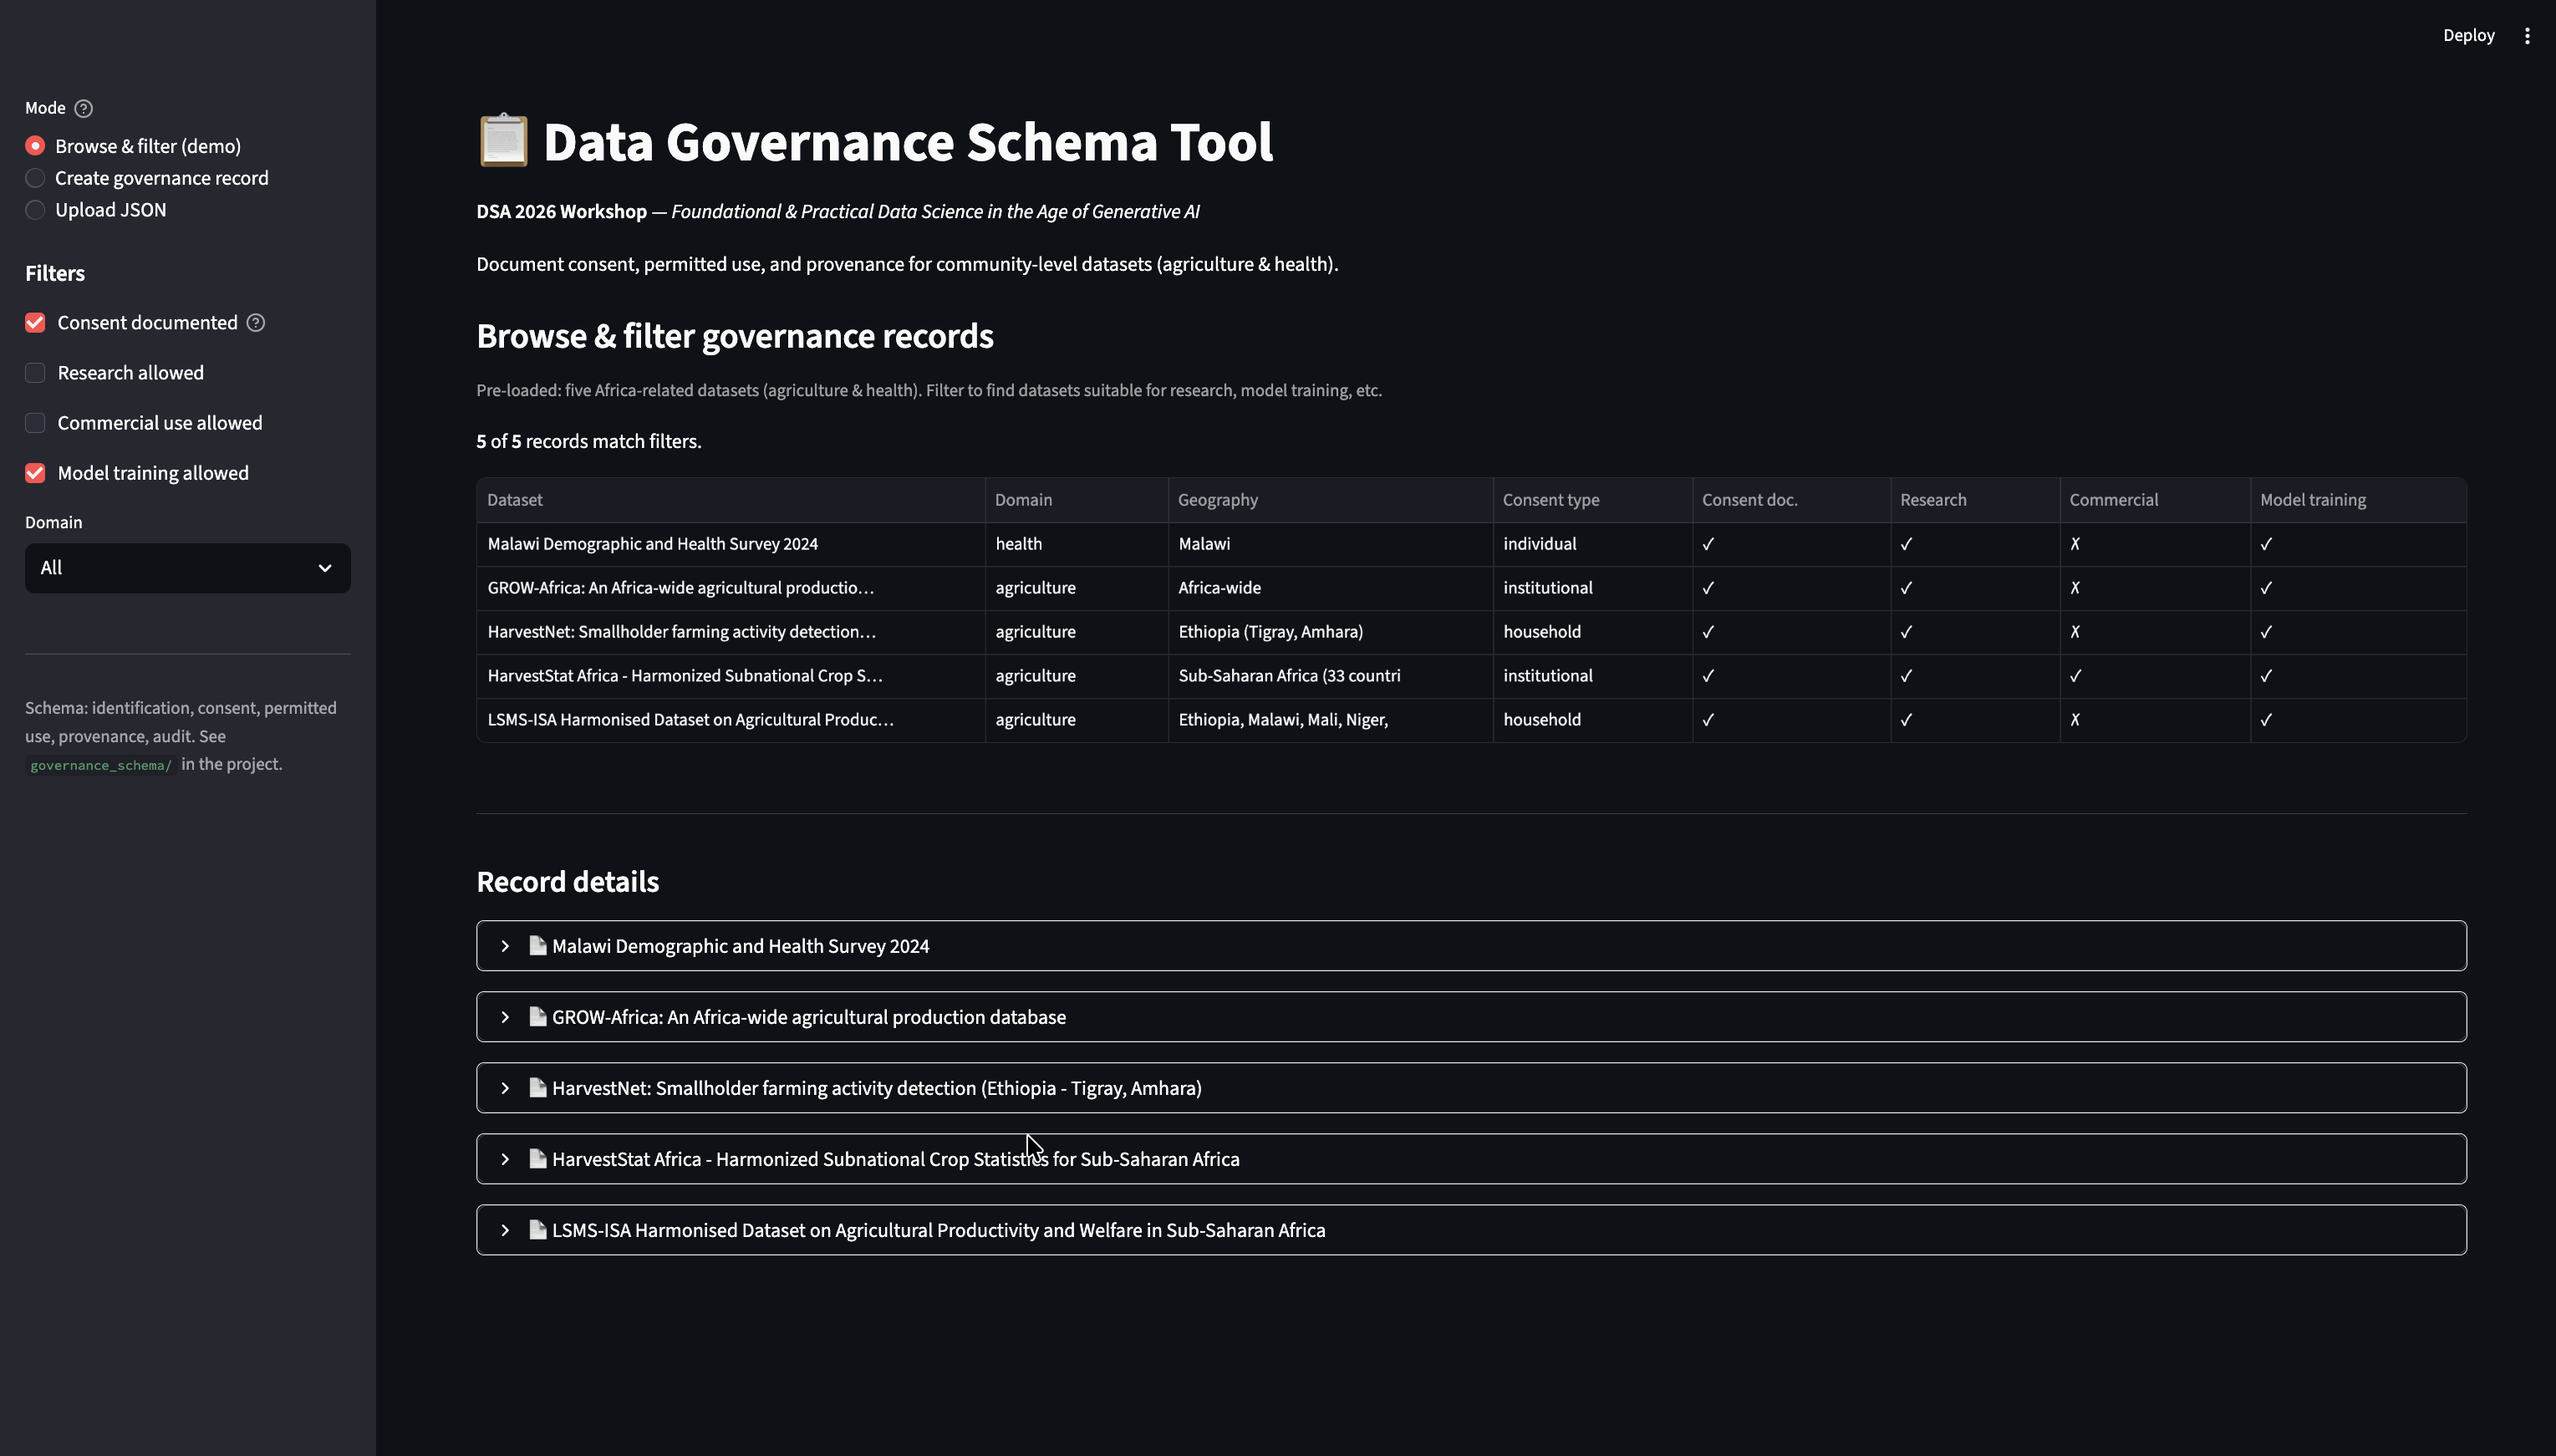
\includegraphics[width=\linewidth]{tool_screenshot_browse.png}
\small\textbf{(a)} Browse and filter.
\end{minipage}
\hfill
\begin{minipage}{0.48\textwidth}
\centering
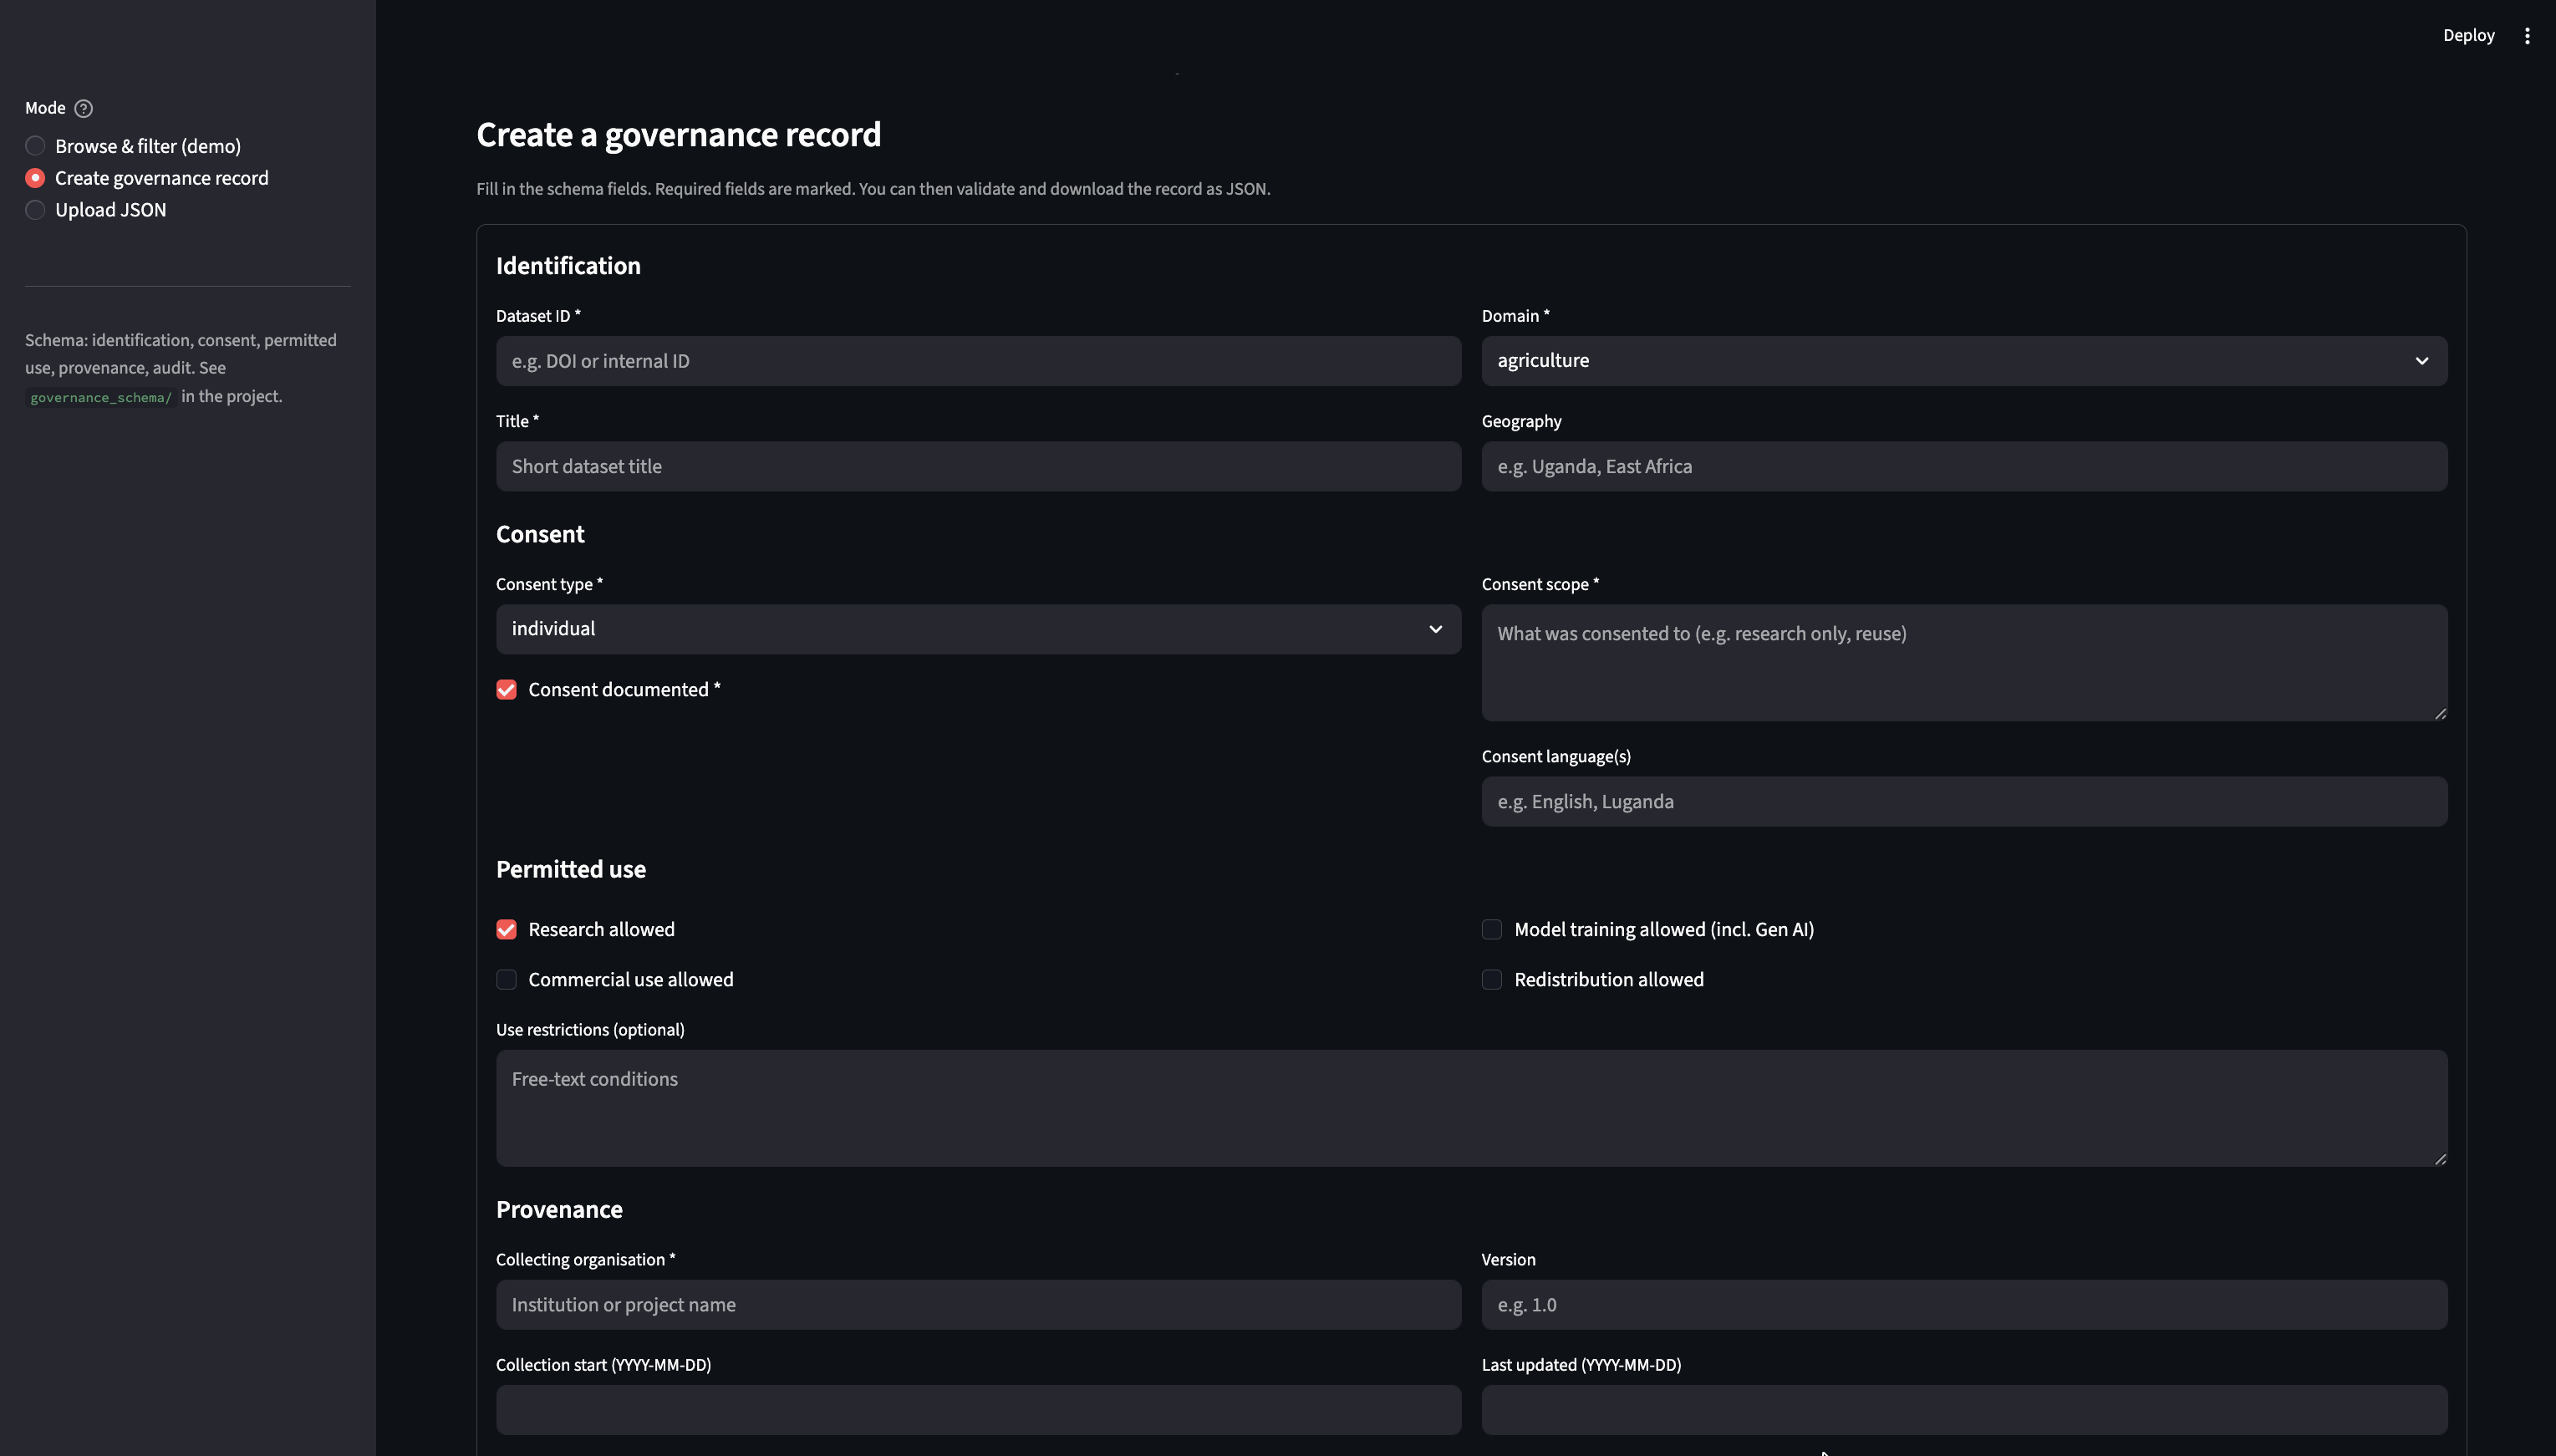
\includegraphics[width=\linewidth]{tool_screenshot_form.png}
\small\textbf{(b)} Create governance record.
\end{minipage}
\caption{Streamlit tool: (a) browsing and filtering the five governance records; (b) form for creating a new record.}
\label{fig:tool}
\end{figure*}

\section{Application to Five Africa-Related Datasets}
\label{sec:application}

The schema was applied to five recent, public, Africa-related datasets: three in agriculture (HarvestStat Africa, LSMS-ISA harmonised, GROW-Africa), one in health (Malawi DHS 2024), and one combining agriculture and remote sensing (HarvestNet, Ethiopia). \Cref{tab:application} summarises the resulting governance records.

\begin{table*}[t]
\centering
\caption{Application summary: five datasets and selected governance fields.}
\label{tab:application}
\small
\begin{tabular}{@{}llllccccc@{}}
\toprule
Dataset & Domain & Geography & Consent & Res. & Comm. & ML & Redist. & Doc. \\
\midrule
HarvestStat Africa & Ag & SSA (33) & Inst. & \checkmark & \checkmark & \checkmark & \checkmark & \checkmark \\
LSMS-ISA harmonised & Ag & 7 SSA & HH & \checkmark & $\times$ & \checkmark & $\times$ & \checkmark \\
GROW-Africa & Ag & Africa & Inst. & \checkmark & $\times$ & \checkmark & $\times$ & \checkmark \\
Malawi DHS 2024 & Health & Malawi & Ind. & \checkmark & $\times$ & \checkmark & $\times$ & \checkmark \\
HarvestNet (Ethiopia) & Ag & Ethiopia & HH & \checkmark & $\times$ & \checkmark & $\times$ & \checkmark \\
\bottomrule
\end{tabular}
\end{table*}

HarvestStat Africa \cite{desbureaux2025} offers aggregate subnational crop statistics (574k records, 33 SSA countries) under CC0. Consent is institutional; all uses are permitted. LSMS-ISA harmonised \cite{gourlay2025} is a longitudinal household and plot-level dataset (seven countries, 2008--2024). Consent is at household level; World Bank terms allow research and model training but prohibit commercial use and redistribution of microdata. GROW-Africa \cite{jain2025} is an Africa-wide database of crop yields (535k observations) assembled from multiple sources. The governance record reflects institutional consent, research and model training allowed, and no commercial use or redistribution. Malawi DHS 2024 is a demographic and health survey (22k+ households) with strong governance: individual consent is documented, research and model training are allowed for registered projects, and commercial use and microdata redistribution are prohibited. HarvestNet (Ethiopia) is a smallholder dataset combining remote sensing and ground labels; the record documents household consent and permits research and model training but not commercial use or redistribution.

Across the five records, the schema surfaces clear variation: three consent types (institutional, household, individual), four of five datasets restrict commercial use and redistribution, and all five document consent and allow model training for research. Filtering by these fields is therefore meaningful.

In practice, the schema supports three kinds of use. First, \textbf{filtering for ethical ML}: for example, selecting only datasets where consent is documented and model training is permitted (all five qualify on these criteria; DHS additionally requires registration). Second, \textbf{filtering by domain or geography} (e.g.\ health only, or Ethiopia). Third, \textbf{audit}: provenance and audit fields answer ``who collected, when, and who to contact'' for compliance or reuse decisions.

\section{Discussion}
\label{sec:discussion}

The schema is deliberately minimal and machine-readable, so it can sit alongside existing policies \cite{effoduh2024} and support the kind of guidelines that researchers in SSA have asked for \cite{brown2024,chabilall2024}. Applying it to five diverse datasets shows that consent type and permitted use vary widely, from institutional to household to individual and from fully open (CC0) to restricted. Encoding them in a common way enables filtering and audit without replacing existing terms of use.

Several limitations should be kept in mind. The filled records were produced from public documentation and terms; they are not formally endorsed by data custodians. Real adoption will depend on institutional or national guidelines and on incentives for data collectors to use the template. By making consent and permitted use machine-readable, the schema lowers the governance barrier to responsible ML experimentation while preserving institutional control. Enforcement of terms remains with custodians and legal frameworks. The schema has not yet been validated with data collectors or research ethics committees in Africa; that would be an important next step.

Future work could extend the Streamlit app (e.g.\ a hosted form for collectors), align the schema more closely with African data ethics frameworks \cite{barrett2025} and data justice principles \cite{munung2025}, run adoption pilots with one or two African institutions, and add fields for retention or data minimisation if local regulation requires it.

\section{Conclusion}

This paper introduced a minimal governance schema for community-level datasets that records consent type and scope, permitted use (research, commercial, model training, redistribution), and provenance and audit information. The schema was applied to five recent Africa-related datasets in agriculture and health, and the results show how it supports filtering for ethical downstream ML and audit trails. The schema, template, rationales, filled records, and Streamlit tool are offered as a reusable artifact for practical data governance in the age of generative AI, where reuse and training on community data ought to be traceable and consent-aware.

\bibliographystyle{ieeetr}
\bibliography{references}

\end{multicols}
\end{document}
